\documentclass[../tex_main/NEMO_manual]{subfiles}
\begin{document}
% ================================================================
% Chapter  Vertical Ocean Physics (ZDF)
% ================================================================
\chapter{Vertical Ocean Physics (ZDF)}
\label{chap:ZDF}
\minitoc

%gm% Add here a small introduction to ZDF and naming of the different physics (similar to what have been written for TRA and DYN.


\newpage
$\ $\newline    % force a new ligne


% ================================================================
% Vertical Mixing
% ================================================================
\section{Vertical mixing}
\label{sec:ZDF_zdf}

The discrete form of the ocean subgrid scale physics has been presented in 
\autoref{sec:TRA_zdf} and \autoref{sec:DYN_zdf}. At the surface and bottom boundaries, 
the turbulent fluxes of momentum, heat and salt have to be defined. At the 
surface they are prescribed from the surface forcing (see \autoref{chap:SBC}), 
while at the bottom they are set to zero for heat and salt, unless a geothermal 
flux forcing is prescribed as a bottom boundary condition ($i.e.$ \key{trabbl} 
defined, see \autoref{subsec:TRA_bbc}), and specified through a bottom friction 
parameterisation for momentum (see \autoref{sec:ZDF_bfr}).

In this section we briefly discuss the various choices offered to compute 
the vertical eddy viscosity and diffusivity coefficients, $A_u^{vm}$ , 
$A_v^{vm}$ and $A^{vT}$ ($A^{vS}$), defined at $uw$-, $vw$- and $w$- 
points, respectively (see \autoref{sec:TRA_zdf} and \autoref{sec:DYN_zdf}). These 
coefficients can be assumed to be either constant, or a function of the local 
Richardson number, or computed from a turbulent closure model (either 
TKE or GLS formulation). The computation of these coefficients is initialized 
in the \mdl{zdfini} module and performed in the \mdl{zdfric}, \mdl{zdftke} or 
\mdl{zdfgls} modules. The trends due to the vertical momentum and tracer 
diffusion, including the surface forcing, are computed and added to the 
general trend in the \mdl{dynzdf} and \mdl{trazdf} modules, respectively. 
These trends can be computed using either a forward time stepping scheme 
(namelist parameter \np{ln\_zdfexp}\forcode{ = .true.}) or a backward time stepping 
scheme (\np{ln\_zdfexp}\forcode{ = .false.}) depending on the magnitude of the mixing 
coefficients, and thus of the formulation used (see \autoref{chap:STP}).

% -------------------------------------------------------------------------------------------------------------
%        Constant 
% -------------------------------------------------------------------------------------------------------------
\subsection{Constant (\protect\key{zdfcst})}
\label{subsec:ZDF_cst}
%--------------------------------------------namzdf---------------------------------------------------------

\nlst{namzdf}
%--------------------------------------------------------------------------------------------------------------

Options are defined through the  \ngn{namzdf} namelist variables.
When \key{zdfcst} is defined, the momentum and tracer vertical eddy coefficients 
are set to constant values over the whole ocean. This is the crudest way to define 
the vertical ocean physics. It is recommended that this option is only used in 
process studies, not in basin scale simulations. Typical values used in this case are:
\begin{align*} 
A_u^{vm} = A_v^{vm} &= 1.2\ 10^{-4}~m^2.s^{-1} 	\\
A^{vT} = A^{vS} &= 1.2\ 10^{-5}~m^2.s^{-1}
\end{align*}

These values are set through the \np{rn\_avm0} and \np{rn\_avt0} namelist parameters. 
In all cases, do not use values smaller that those associated with the molecular 
viscosity and diffusivity, that is $\sim10^{-6}~m^2.s^{-1}$ for momentum, 
$\sim10^{-7}~m^2.s^{-1}$ for temperature and $\sim10^{-9}~m^2.s^{-1}$ for salinity.


% -------------------------------------------------------------------------------------------------------------
%        Richardson Number Dependent
% -------------------------------------------------------------------------------------------------------------
\subsection{Richardson number dependent (\protect\key{zdfric})}
\label{subsec:ZDF_ric}

%--------------------------------------------namric---------------------------------------------------------

\nlst{namzdf_ric}
%--------------------------------------------------------------------------------------------------------------

When \key{zdfric} is defined, a local Richardson number dependent formulation 
for the vertical momentum and tracer eddy coefficients is set through the  \ngn{namzdf\_ric} 
namelist variables.The vertical mixing 
coefficients are diagnosed from the large scale variables computed by the model. 
\textit{In situ} measurements have been used to link vertical turbulent activity to 
large scale ocean structures. The hypothesis of a mixing mainly maintained by the 
growth of Kelvin-Helmholtz like instabilities leads to a dependency between the 
vertical eddy coefficients and the local Richardson number ($i.e.$ the 
ratio of stratification to vertical shear). Following \citet{Pacanowski_Philander_JPO81}, the following 
formulation has been implemented:
\begin{equation} \label{eq:zdfric}
   \left\{      \begin{aligned}
         A^{vT} &= \frac {A_{ric}^{vT}}{\left( 1+a \; Ri \right)^n} + A_b^{vT}       \\
         A^{vm} &= \frac{A^{vT}        }{\left( 1+ a \;Ri  \right)   } + A_b^{vm}
   \end{aligned}    \right.
\end{equation}
where $Ri = N^2 / \left(\partial_z \textbf{U}_h \right)^2$ is the local Richardson 
number, $N$ is the local Brunt-Vais\"{a}l\"{a} frequency (see \autoref{subsec:TRA_bn2}), 
$A_b^{vT} $ and $A_b^{vm}$ are the constant background values set as in the 
constant case (see \autoref{subsec:ZDF_cst}), and $A_{ric}^{vT} = 10^{-4}~m^2.s^{-1}$ 
is the maximum value that can be reached by the coefficient when $Ri\leq 0$, 
$a=5$ and $n=2$. The last three values can be modified by setting the 
\np{rn\_avmri}, \np{rn\_alp} and \np{nn\_ric} namelist parameters, respectively.

A simple mixing-layer model to transfer and dissipate the atmospheric
 forcings (wind-stress and buoyancy fluxes) can be activated setting 
the \np{ln\_mldw}\forcode{ = .true.} in the namelist.

In this case, the local depth of turbulent wind-mixing or "Ekman depth"
 $h_{e}(x,y,t)$ is evaluated and the vertical eddy coefficients prescribed within this layer.

This depth is assumed proportional to the "depth of frictional influence" that is limited by rotation:
\begin{equation}
         h_{e} = Ek \frac {u^{*}} {f_{0}}  	\\
\end{equation}
where, $Ek$ is an empirical parameter, $u^{*}$ is the friction velocity and $f_{0}$ is the Coriolis 
parameter.

In this similarity height relationship, the turbulent friction velocity:
\begin{equation}
         u^{*} = \sqrt \frac {|\tau|} {\rho_o}  	\\
\end{equation}

is computed from the wind stress vector $|\tau|$ and the reference density $ \rho_o$.
The final $h_{e}$ is further constrained by the adjustable bounds \np{rn\_mldmin} and \np{rn\_mldmax}.
Once $h_{e}$ is computed, the vertical eddy coefficients within $h_{e}$ are set to 
the empirical values \np{rn\_wtmix} and \np{rn\_wvmix} \citep{Lermusiaux2001}.

% -------------------------------------------------------------------------------------------------------------
%        TKE Turbulent Closure Scheme 
% -------------------------------------------------------------------------------------------------------------
\subsection{TKE turbulent closure scheme (\protect\key{zdftke})}
\label{subsec:ZDF_tke}

%--------------------------------------------namzdf_tke--------------------------------------------------

\nlst{namzdf_tke}
%--------------------------------------------------------------------------------------------------------------

The vertical eddy viscosity and diffusivity coefficients are computed from a TKE 
turbulent closure model based on a prognostic equation for $\bar{e}$, the turbulent 
kinetic energy, and a closure assumption for the turbulent length scales. This 
turbulent closure model has been developed by \citet{Bougeault1989} in the 
atmospheric case, adapted by \citet{Gaspar1990} for the oceanic case, and 
embedded in OPA, the ancestor of NEMO, by \citet{Blanke1993} for equatorial Atlantic 
simulations. Since then, significant modifications have been introduced by 
\citet{Madec1998} in both the implementation and the formulation of the mixing 
length scale. The time evolution of $\bar{e}$ is the result of the production of 
$\bar{e}$ through vertical shear, its destruction through stratification, its vertical 
diffusion, and its dissipation of \citet{Kolmogorov1942} type:
\begin{equation} \label{eq:zdftke_e}
\frac{\partial \bar{e}}{\partial t} = 
\frac{K_m}{{e_3}^2 }\;\left[ {\left( {\frac{\partial u}{\partial k}} \right)^2
				        +\left( {\frac{\partial v}{\partial k}} \right)^2} \right]
-K_\rho\,N^2
+\frac{1}{e_3}	\;\frac{\partial }{\partial k}\left[ {\frac{A^{vm}}{e_3 }
				\;\frac{\partial \bar{e}}{\partial k}} \right]
- c_\epsilon \;\frac{\bar {e}^{3/2}}{l_\epsilon }
\end{equation}
\begin{equation} \label{eq:zdftke_kz}
   \begin{split}
         K_m &= C_k\  l_k\  \sqrt {\bar{e}\; }  	\\
         K_\rho &= A^{vm} / P_{rt}
   \end{split}
\end{equation}
where $N$ is the local Brunt-Vais\"{a}l\"{a} frequency (see \autoref{subsec:TRA_bn2}), 
$l_{\epsilon }$ and $l_{\kappa }$ are the dissipation and mixing length scales, 
$P_{rt}$ is the Prandtl number, $K_m$ and $K_\rho$ are the vertical eddy viscosity 
and diffusivity coefficients. The constants $C_k =  0.1$ and $C_\epsilon = \sqrt {2} /2$  
$\approx 0.7$ are designed to deal with vertical mixing at any depth \citep{Gaspar1990}. 
They are set through namelist parameters \np{nn\_ediff} and \np{nn\_ediss}. 
$P_{rt}$ can be set to unity or, following \citet{Blanke1993}, be a function 
of the local Richardson number, $R_i$:
\begin{align*} \label{eq:prt}
P_{rt} = \begin{cases}
                    \ \ \ 1 &      \text{if $\ R_i \leq 0.2$} 	\\
                    5\,R_i &      \text{if $\ 0.2 \leq R_i \leq 2$} 	\\
                    \ \ 10 &      \text{if $\ 2 \leq R_i$} 
            \end{cases}
\end{align*}
Options are defined through the  \ngn{namzdfy\_tke} namelist variables.
The choice of $P_{rt}$ is controlled by the \np{nn\_pdl} namelist variable.

At the sea surface, the value of $\bar{e}$ is prescribed from the wind 
stress field as $\bar{e}_o = e_{bb} |\tau| / \rho_o$, with $e_{bb}$ the \np{rn\_ebb} 
namelist parameter. The default value of $e_{bb}$ is 3.75. \citep{Gaspar1990}), 
however a much larger value can be used when taking into account the 
surface wave breaking (see below Eq. \autoref{eq:ZDF_Esbc}). 
The bottom value of TKE is assumed to be equal to the value of the level just above. 
The time integration of the $\bar{e}$ equation may formally lead to negative values 
because the numerical scheme does not ensure its positivity. To overcome this 
problem, a cut-off in the minimum value of $\bar{e}$ is used (\np{rn\_emin} 
namelist parameter). Following \citet{Gaspar1990}, the cut-off value is set 
to $\sqrt{2}/2~10^{-6}~m^2.s^{-2}$. This allows the subsequent formulations 
to match that of \citet{Gargett1984} for the diffusion in the thermocline and 
deep ocean :  $K_\rho = 10^{-3} / N$. 
In addition, a cut-off is applied on $K_m$ and $K_\rho$ to avoid numerical 
instabilities associated with too weak vertical diffusion. They must be 
specified at least larger than the molecular values, and are set through 
\np{rn\_avm0} and \np{rn\_avt0} (namzdf namelist, see \autoref{subsec:ZDF_cst}).

\subsubsection{Turbulent length scale}
For computational efficiency, the original formulation of the turbulent length 
scales proposed by \citet{Gaspar1990} has been simplified. Four formulations 
are proposed, the choice of which is controlled by the \np{nn\_mxl} namelist 
parameter. The first two are based on the following first order approximation 
\citep{Blanke1993}:
\begin{equation} \label{eq:tke_mxl0_1}
l_k = l_\epsilon = \sqrt {2 \bar{e}\; } / N
\end{equation}
which is valid in a stable stratified region with constant values of the Brunt-
Vais\"{a}l\"{a} frequency. The resulting length scale is bounded by the distance 
to the surface or to the bottom (\np{nn\_mxl}\forcode{ = 0}) or by the local vertical scale factor 
(\np{nn\_mxl}\forcode{ = 1}). \citet{Blanke1993} notice that this simplification has two major 
drawbacks: it makes no sense for locally unstable stratification and the 
computation no longer uses all the information contained in the vertical density 
profile. To overcome these drawbacks, \citet{Madec1998} introduces the 
\np{nn\_mxl}\forcode{ = 2..3} cases, which add an extra assumption concerning the vertical 
gradient of the computed length scale. So, the length scales are first evaluated 
as in \autoref{eq:tke_mxl0_1} and then bounded such that:
\begin{equation} \label{eq:tke_mxl_constraint}
\frac{1}{e_3 }\left| {\frac{\partial l}{\partial k}} \right| \leq 1
\qquad \text{with }\  l =  l_k = l_\epsilon
\end{equation}
\autoref{eq:tke_mxl_constraint} means that the vertical variations of the length 
scale cannot be larger than the variations of depth. It provides a better 
approximation of the \citet{Gaspar1990} formulation while being much less 
time consuming. In particular, it allows the length scale to be limited not only 
by the distance to the surface or to the ocean bottom but also by the distance 
to a strongly stratified portion of the water column such as the thermocline 
(\autoref{fig:mixing_length}). In order to impose the \autoref{eq:tke_mxl_constraint} 
constraint, we introduce two additional length scales: $l_{up}$ and $l_{dwn}$, 
the upward and downward length scales, and evaluate the dissipation and 
mixing length scales as (and note that here we use numerical indexing):
%>>>>>>>>>>>>>>>>>>>>>>>>>>>>
\begin{figure}[!t] \begin{center}
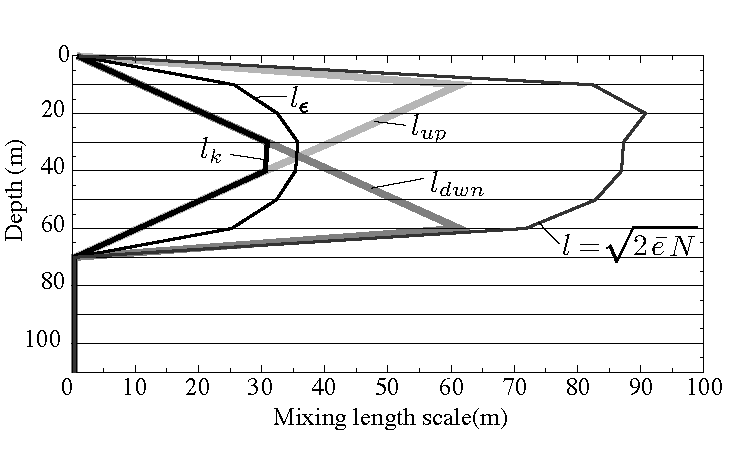
\includegraphics[width=1.00\textwidth]{Fig_mixing_length}
\caption{ \protect\label{fig:mixing_length} 
Illustration of the mixing length computation. }
\end{center}  
\end{figure}
%>>>>>>>>>>>>>>>>>>>>>>>>>>>>
\begin{equation} \label{eq:tke_mxl2}
\begin{aligned}
 l_{up\ \ }^{(k)} &= \min \left(  l^{(k)} \ , \ l_{up}^{(k+1)} + e_{3t}^{(k)}\ \ \ \;  \right)
    \quad &\text{ from $k=1$ to $jpk$ }\ \\
 l_{dwn}^{(k)} &= \min \left(  l^{(k)} \ , \ l_{dwn}^{(k-1)} + e_{3t}^{(k-1)}  \right)   
    \quad &\text{ from $k=jpk$ to $1$ }\ \\
\end{aligned}
\end{equation}
where $l^{(k)}$ is computed using \autoref{eq:tke_mxl0_1}, 
$i.e.$ $l^{(k)} = \sqrt {2 {\bar e}^{(k)} / {N^2}^{(k)} }$.

In the \np{nn\_mxl}\forcode{ = 2} case, the dissipation and mixing length scales take the same 
value: $ l_k=  l_\epsilon = \min \left(\ l_{up} \;,\;  l_{dwn}\ \right)$, while in the 
\np{nn\_mxl}\forcode{ = 3} case, the dissipation and mixing turbulent length scales are give 
as in \citet{Gaspar1990}:
\begin{equation} \label{eq:tke_mxl_gaspar}
\begin{aligned}
& l_k          = \sqrt{\  l_{up} \ \ l_{dwn}\ }  	\\
& l_\epsilon = \min \left(\ l_{up} \;,\;  l_{dwn}\ \right) 
\end{aligned}
\end{equation}

At the ocean surface, a non zero length scale is set through the  \np{rn\_mxl0} namelist 
parameter. Usually the surface scale is given by $l_o = \kappa \,z_o$ 
where $\kappa = 0.4$ is von Karman's constant and $z_o$ the roughness 
parameter of the surface. Assuming $z_o=0.1$~m \citep{Craig_Banner_JPO94} 
leads to a 0.04~m, the default value of \np{rn\_mxl0}. In the ocean interior 
a minimum length scale is set to recover the molecular viscosity when $\bar{e}$ 
reach its minimum value ($1.10^{-6}= C_k\, l_{min} \,\sqrt{\bar{e}_{min}}$ ).


\subsubsection{Surface wave breaking parameterization}
%-----------------------------------------------------------------------%
Following \citet{Mellor_Blumberg_JPO04}, the TKE turbulence closure model has been modified 
to include the effect of surface wave breaking energetics. This results in a reduction of summertime 
surface temperature when the mixed layer is relatively shallow. The \citet{Mellor_Blumberg_JPO04} 
modifications acts on surface length scale and TKE values and air-sea drag coefficient. 
The latter concerns the bulk formulea and is not discussed here. 

Following \citet{Craig_Banner_JPO94}, the boundary condition on surface TKE value is :
\begin{equation}  \label{eq:ZDF_Esbc}
\bar{e}_o = \frac{1}{2}\,\left(  15.8\,\alpha_{CB} \right)^{2/3} \,\frac{|\tau|}{\rho_o}
\end{equation}
where $\alpha_{CB}$ is the \citet{Craig_Banner_JPO94} constant of proportionality 
which depends on the ''wave age'', ranging from 57 for mature waves to 146 for 
younger waves \citep{Mellor_Blumberg_JPO04}. 
The boundary condition on the turbulent length scale follows the Charnock's relation:
\begin{equation} \label{eq:ZDF_Lsbc}
l_o = \kappa \beta \,\frac{|\tau|}{g\,\rho_o}
\end{equation}
where $\kappa=0.40$ is the von Karman constant, and $\beta$ is the Charnock's constant.
\citet{Mellor_Blumberg_JPO04} suggest $\beta = 2.10^{5}$ the value chosen by \citet{Stacey_JPO99}
citing observation evidence, and $\alpha_{CB} = 100$ the Craig and Banner's value.
As the surface boundary condition on TKE is prescribed through $\bar{e}_o = e_{bb} |\tau| / \rho_o$, 
with $e_{bb}$ the \np{rn\_ebb} namelist parameter, setting \np{rn\_ebb}\forcode{ = 67.83} corresponds 
to $\alpha_{CB} = 100$. Further setting  \np{ln\_mxl0} to true applies \autoref{eq:ZDF_Lsbc} 
as surface boundary condition on length scale, with $\beta$ hard coded to the Stacey's value.
Note that a minimal threshold of \np{rn\_emin0}$=10^{-4}~m^2.s^{-2}$ (namelist parameters) 
is applied on surface $\bar{e}$ value.


\subsubsection{Langmuir cells}
%--------------------------------------%
Langmuir circulations (LC) can be described as ordered large-scale vertical motions 
in the surface layer of the oceans. Although LC have nothing to do with convection, 
the circulation pattern is rather similar to so-called convective rolls in the atmospheric 
boundary layer. The detailed physics behind LC is described in, for example, 
\citet{Craik_Leibovich_JFM76}. The prevailing explanation is that LC arise from 
a nonlinear interaction between the Stokes drift and wind drift currents. 

Here we introduced in the TKE turbulent closure the simple parameterization of 
Langmuir circulations proposed by \citep{Axell_JGR02} for a $k-\epsilon$ turbulent closure. 
The parameterization, tuned against large-eddy simulation, includes the whole effect
of LC in an extra source terms of TKE, $P_{LC}$.
The presence of $P_{LC}$ in \autoref{eq:zdftke_e}, the TKE equation, is controlled 
by setting \np{ln\_lc} to \forcode{.true.} in the namtke namelist.
 
By making an analogy with the characteristic convective velocity scale 
($e.g.$, \citet{D'Alessio_al_JPO98}), $P_{LC}$ is assumed to be : 
\begin{equation}
P_{LC}(z) = \frac{w_{LC}^3(z)}{H_{LC}}
\end{equation}
where $w_{LC}(z)$ is the vertical velocity profile of LC, and $H_{LC}$ is the LC depth.
With no information about the wave field, $w_{LC}$ is assumed to be proportional to 
the Stokes drift $u_s = 0.377\,\,|\tau|^{1/2}$, where $|\tau|$ is the surface wind stress module 
\footnote{Following \citet{Li_Garrett_JMR93}, the surface Stoke drift velocity
may be expressed as $u_s =  0.016 \,|U_{10m}|$. Assuming an air density of 
$\rho_a=1.22 \,Kg/m^3$ and a drag coefficient of $1.5~10^{-3}$ give the expression 
used of $u_s$ as a function of the module of surface stress}. 
For the vertical variation, $w_{LC}$ is assumed to be zero at the surface as well as 
at a finite depth $H_{LC}$ (which is often close to the mixed layer depth), and simply 
varies as a sine function in between (a first-order profile for the Langmuir cell structures). 
The resulting expression for $w_{LC}$ is :
\begin{equation}
w_{LC}  = \begin{cases}
                   c_{LC} \,u_s \,\sin(- \pi\,z / H_{LC} )    &      \text{if $-z \leq H_{LC}$} 	\\
                   0                 				 &      \text{otherwise} 
                 \end{cases}
\end{equation}
where $c_{LC} = 0.15$ has been chosen by \citep{Axell_JGR02} as a good compromise 
to fit LES data. The chosen value yields maximum vertical velocities $w_{LC}$ of the order 
of a few centimeters per second. The value of $c_{LC}$ is set through the \np{rn\_lc} 
namelist parameter, having in mind that it should stay between 0.15 and 0.54 \citep{Axell_JGR02}. 

The $H_{LC}$ is estimated in a similar way as the turbulent length scale of TKE equations:
$H_{LC}$ is depth to which a water parcel with kinetic energy due to Stoke drift
can reach on its own by converting its kinetic energy to potential energy, according to 
\begin{equation}
- \int_{-H_{LC}}^0 { N^2\;z  \;dz} = \frac{1}{2} u_s^2
\end{equation}


\subsubsection{Mixing just below the mixed layer}
%--------------------------------------------------------------%

Vertical mixing parameterizations commonly used in ocean general circulation models 
tend to produce mixed-layer depths that are too shallow during summer months and windy conditions.
This bias is particularly acute over the Southern Ocean. 
To overcome this systematic bias, an ad hoc parameterization is introduced into the TKE scheme  \cite{Rodgers_2014}. 
The parameterization is an empirical one, $i.e.$ not derived from theoretical considerations, 
but rather is meant to account for observed processes that affect the density structure of 
the ocean’s planetary boundary layer that are not explicitly captured by default in the TKE scheme 
($i.e.$ near-inertial oscillations and ocean swells and waves).

When using this parameterization ($i.e.$ when \np{nn\_etau}\forcode{ = 1}), the TKE input to the ocean ($S$) 
imposed by the winds in the form of near-inertial oscillations, swell and waves is parameterized 
by \autoref{eq:ZDF_Esbc} the standard TKE surface boundary condition, plus a depth depend one given by:
\begin{equation}  \label{eq:ZDF_Ehtau}
S = (1-f_i) \; f_r \; e_s \; e^{-z / h_\tau} 
\end{equation}
where 
$z$ is the depth,  
$e_s$ is TKE surface boundary condition, 
$f_r$ is the fraction of the surface TKE that penetrate in the ocean, 
$h_\tau$ is a vertical mixing length scale that controls exponential shape of the penetration, 
and $f_i$ is the ice concentration (no penetration if $f_i=1$, that is if the ocean is entirely 
covered by sea-ice).
The value of $f_r$, usually a few percents, is specified through \np{rn\_efr} namelist parameter. 
The vertical mixing length scale, $h_\tau$, can be set as a 10~m uniform value (\np{nn\_etau}\forcode{ = 0}) 
or a latitude dependent value (varying from 0.5~m at the Equator to a maximum value of 30~m 
at high latitudes (\np{nn\_etau}\forcode{ = 1}). 

Note that two other option existe, \np{nn\_etau}\forcode{ = 2..3}. They correspond to applying 
\autoref{eq:ZDF_Ehtau} only at the base of the mixed layer, or to using the high frequency part 
of the stress to evaluate the fraction of TKE that penetrate the ocean. 
Those two options are obsolescent features introduced for test purposes.
They will be removed in the next release. 



% from Burchard et al OM 2008 : 
% the most critical process not reproduced by statistical turbulence models is the activity of 
% internal waves and their interaction with turbulence. After the Reynolds decomposition, 
% internal waves are in principle included in the RANS equations, but later partially 
% excluded by the hydrostatic assumption and the model resolution. 
% Thus far, the representation of internal wave mixing in ocean models has been relatively crude 
% (e.g. Mellor, 1989; Large et al., 1994; Meier, 2001; Axell, 2002; St. Laurent and Garrett, 2002).



% -------------------------------------------------------------------------------------------------------------
%        TKE discretization considerations
% -------------------------------------------------------------------------------------------------------------
\subsection{TKE discretization considerations (\protect\key{zdftke})}
\label{subsec:ZDF_tke_ene}

%>>>>>>>>>>>>>>>>>>>>>>>>>>>>
\begin{figure}[!t]   \begin{center}
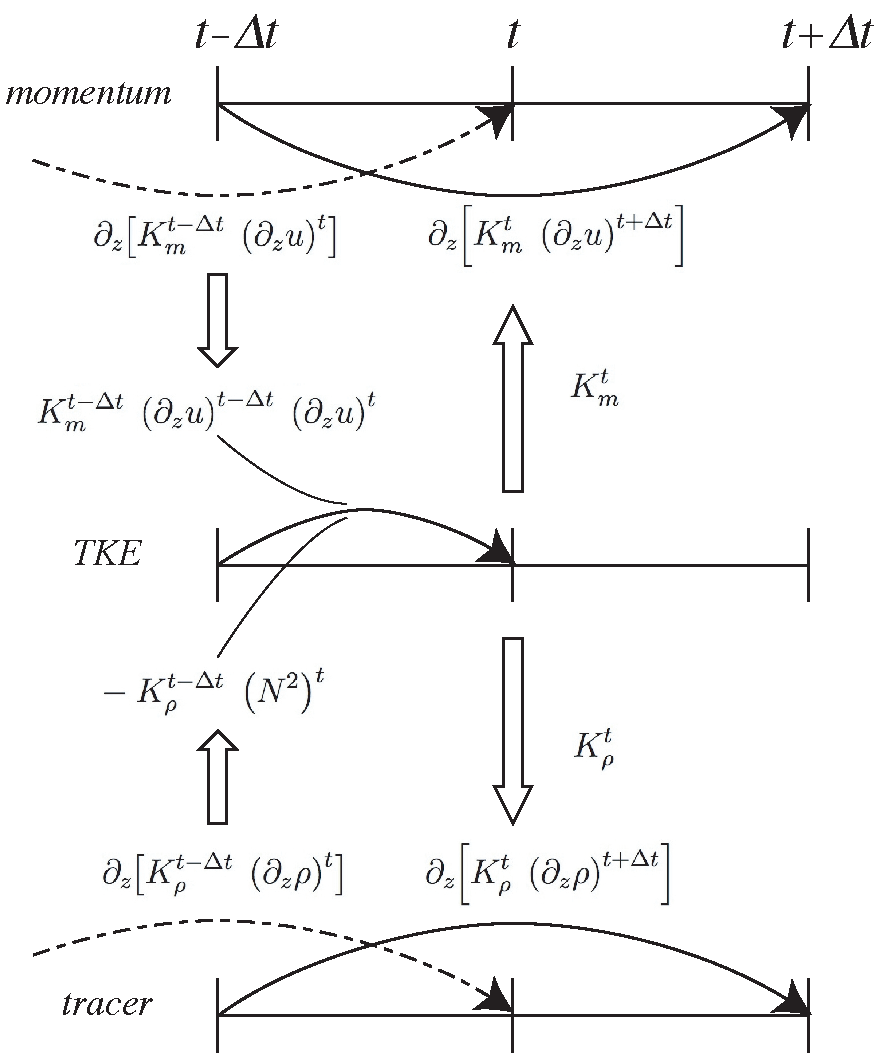
\includegraphics[width=1.00\textwidth]{Fig_ZDF_TKE_time_scheme}
\caption{ \protect\label{fig:TKE_time_scheme} 
Illustration of the TKE time integration and its links to the momentum and tracer time integration. }
\end{center}  
\end{figure}
%>>>>>>>>>>>>>>>>>>>>>>>>>>>>

The production of turbulence by vertical shear (the first term of the right hand side 
of \autoref{eq:zdftke_e}) should balance the loss of kinetic energy associated with
the vertical momentum diffusion (first line in \autoref{eq:PE_zdf}). To do so a special care 
have to be taken for both the time and space discretization of the TKE equation 
\citep{Burchard_OM02,Marsaleix_al_OM08}.

Let us first address the time stepping issue. \autoref{fig:TKE_time_scheme} shows 
how the two-level Leap-Frog time stepping of the momentum and tracer equations interplays 
with the one-level forward time stepping of TKE equation. With this framework, the total loss 
of kinetic energy (in 1D for the demonstration) due to the vertical momentum diffusion is 
obtained by multiplying this quantity by $u^t$ and summing the result vertically:   
\begin{equation} \label{eq:energ1}
\begin{split}
\int_{-H}^{\eta}  u^t \,\partial_z &\left( {K_m}^t \,(\partial_z u)^{t+\rdt}  \right) \,dz   \\
&= \Bigl[  u^t \,{K_m}^t \,(\partial_z u)^{t+\rdt} \Bigr]_{-H}^{\eta}          
 - \int_{-H}^{\eta}{ {K_m}^t \,\partial_z{u^t} \,\partial_z u^{t+\rdt} \,dz }
\end{split}
\end{equation}
Here, the vertical diffusion of momentum is discretized backward in time 
with a coefficient, $K_m$, known at time $t$ (\autoref{fig:TKE_time_scheme}), 
as it is required when using the TKE scheme (see \autoref{sec:STP_forward_imp}). 
The first term of the right hand side of \autoref{eq:energ1} represents the kinetic energy 
transfer at the surface (atmospheric forcing) and at the bottom (friction effect). 
The second term is always negative. It is the dissipation rate of kinetic energy, 
and thus minus the shear production rate of $\bar{e}$. \autoref{eq:energ1} 
implies that, to be energetically consistent, the production rate of $\bar{e}$ 
used to compute $(\bar{e})^t$ (and thus ${K_m}^t$) should be expressed as 
${K_m}^{t-\rdt}\,(\partial_z u)^{t-\rdt} \,(\partial_z u)^t$ (and not by the more straightforward 
$K_m \left( \partial_z u \right)^2$ expression taken at time $t$ or $t-\rdt$).

A similar consideration applies on the destruction rate of $\bar{e}$ due to stratification 
(second term of the right hand side of \autoref{eq:zdftke_e}). This term 
must balance the input of potential energy resulting from vertical mixing. 
The rate of change of potential energy (in 1D for the demonstration) due vertical 
mixing is obtained by multiplying vertical density diffusion 
tendency by $g\,z$ and and summing the result vertically:
\begin{equation} \label{eq:energ2}
\begin{split}
\int_{-H}^{\eta} g\,z\,\partial_z &\left( {K_\rho}^t \,(\partial_k \rho)^{t+\rdt}   \right) \,dz    \\
&= \Bigl[  g\,z \,{K_\rho}^t \,(\partial_z \rho)^{t+\rdt} \Bigr]_{-H}^{\eta}  
   - \int_{-H}^{\eta}{ g \,{K_\rho}^t \,(\partial_k \rho)^{t+\rdt} } \,dz   \\
&= - \Bigl[  z\,{K_\rho}^t \,(N^2)^{t+\rdt} \Bigr]_{-H}^{\eta}
+ \int_{-H}^{\eta}{  \rho^{t+\rdt} \, {K_\rho}^t \,(N^2)^{t+\rdt} \,dz  }
\end{split}
\end{equation}
where we use $N^2 = -g \,\partial_k \rho / (e_3 \rho)$. 
The first term of the right hand side of \autoref{eq:energ2}  is always zero 
because there is no diffusive flux through the ocean surface and bottom). 
The second term is minus the destruction rate of  $\bar{e}$ due to stratification. 
Therefore \autoref{eq:energ1} implies that, to be energetically consistent, the product 
${K_\rho}^{t-\rdt}\,(N^2)^t$ should be used in \autoref{eq:zdftke_e}, the TKE equation.

Let us now address the space discretization issue. 
The vertical eddy coefficients are defined at $w$-point whereas the horizontal velocity 
components are in the centre of the side faces of a $t$-box in staggered C-grid 
(\autoref{fig:cell}). A space averaging is thus required to obtain the shear TKE production term.
By redoing the \autoref{eq:energ1} in the 3D case, it can be shown that the product of 
eddy coefficient by the shear at $t$ and $t-\rdt$ must be performed prior to the averaging.
Furthermore, the possible time variation of $e_3$ (\key{vvl} case) have to be taken into 
account.

The above energetic considerations leads to 
the following final discrete form for the TKE equation:
\begin{equation} \label{eq:zdftke_ene}
\begin{split}
\frac { (\bar{e})^t - (\bar{e})^{t-\rdt} } {\rdt}  \equiv  
\Biggl\{ \Biggr.
  &\overline{ \left( \left(\overline{K_m}^{\,i+1/2}\right)^{t-\rdt} \,\frac{\delta_{k+1/2}[u^{t+\rdt}]}{{e_3u}^{t+\rdt} } 
                                                                              \ \frac{\delta_{k+1/2}[u^ t         ]}{{e_3u}^ t          }  \right) }^{\,i} \\
+&\overline{  \left( \left(\overline{K_m}^{\,j+1/2}\right)^{t-\rdt} \,\frac{\delta_{k+1/2}[v^{t+\rdt}]}{{e_3v}^{t+\rdt} } 
                                                                               \ \frac{\delta_{k+1/2}[v^ t         ]}{{e_3v}^ t          }  \right) }^{\,j} 
\Biggr. \Biggr\}   \\
%
- &{K_\rho}^{t-\rdt}\,{(N^2)^t}    \\
%
+&\frac{1}{{e_3w}^{t+\rdt}}  \;\delta_{k+1/2} \left[   {K_m}^{t-\rdt} \,\frac{\delta_{k}[(\bar{e})^{t+\rdt}]} {{e_3w}^{t+\rdt}}   \right]   \\
%
- &c_\epsilon \; \left( \frac{\sqrt{\bar {e}}}{l_\epsilon}\right)^{t-\rdt}\,(\bar {e})^{t+\rdt}
\end{split}
\end{equation}
where the last two terms in \autoref{eq:zdftke_ene} (vertical diffusion and Kolmogorov dissipation) 
are time stepped using a backward scheme (see\autoref{sec:STP_forward_imp}). 
Note that the Kolmogorov term has been linearized in time in order to render 
the implicit computation possible. The restart of the TKE scheme 
requires the storage of $\bar {e}$, $K_m$, $K_\rho$ and $l_\epsilon$ as they all appear in 
the right hand side of \autoref{eq:zdftke_ene}. For the latter, it is in fact 
the ratio $\sqrt{\bar{e}}/l_\epsilon$ which is stored. 

% -------------------------------------------------------------------------------------------------------------
%        GLS Generic Length Scale Scheme 
% -------------------------------------------------------------------------------------------------------------
\subsection{GLS: Generic Length Scale (\protect\key{zdfgls})}
\label{subsec:ZDF_gls}

%--------------------------------------------namzdf_gls---------------------------------------------------------

\nlst{namzdf_gls}
%--------------------------------------------------------------------------------------------------------------

The Generic Length Scale (GLS) scheme is a turbulent closure scheme based on 
two prognostic equations: one for the turbulent kinetic energy $\bar {e}$, and another 
for the generic length scale, $\psi$ \citep{Umlauf_Burchard_JMS03, Umlauf_Burchard_CSR05}. 
This later variable is defined as : $\psi = {C_{0\mu}}^{p} \ {\bar{e}}^{m} \ l^{n}$, 
where the triplet $(p, m, n)$ value given in Tab.\autoref{tab:GLS} allows to recover 
a number of well-known turbulent closures ($k$-$kl$ \citep{Mellor_Yamada_1982}, 
$k$-$\epsilon$ \citep{Rodi_1987}, $k$-$\omega$ \citep{Wilcox_1988} 
among others \citep{Umlauf_Burchard_JMS03,Kantha_Carniel_CSR05}). 
The GLS scheme is given by the following set of equations:
\begin{equation} \label{eq:zdfgls_e}
\frac{\partial \bar{e}}{\partial t} = 
\frac{K_m}{\sigma_e e_3 }\;\left[ {\left( \frac{\partial u}{\partial k} \right)^2
                                                   +\left( \frac{\partial v}{\partial k} \right)^2} \right]
-K_\rho \,N^2
+\frac{1}{e_3}\,\frac{\partial}{\partial k} \left[ \frac{K_m}{e_3}\,\frac{\partial \bar{e}}{\partial k} \right]
- \epsilon
\end{equation}

\begin{equation} \label{eq:zdfgls_psi}
   \begin{split}
\frac{\partial \psi}{\partial t} =& \frac{\psi}{\bar{e}} \left\{
\frac{C_1\,K_m}{\sigma_{\psi} {e_3}}\;\left[ {\left( \frac{\partial u}{\partial k} \right)^2
                                                                   +\left( \frac{\partial v}{\partial k} \right)^2} \right]
- C_3 \,K_\rho\,N^2   - C_2 \,\epsilon \,Fw   \right\}             \\
&+\frac{1}{e_3}  \;\frac{\partial }{\partial k}\left[ {\frac{K_m}{e_3 }
                                  \;\frac{\partial \psi}{\partial k}} \right]\;
   \end{split}
\end{equation}

\begin{equation} \label{eq:zdfgls_kz}
   \begin{split}
         K_m    &= C_{\mu} \ \sqrt {\bar{e}} \ l         \\
         K_\rho &= C_{\mu'}\ \sqrt {\bar{e}} \ l
   \end{split}
\end{equation}

\begin{equation} \label{eq:zdfgls_eps}
{\epsilon} = C_{0\mu} \,\frac{\bar {e}^{3/2}}{l} \;
\end{equation}
where $N$ is the local Brunt-Vais\"{a}l\"{a} frequency (see \autoref{subsec:TRA_bn2}) 
and $\epsilon$ the dissipation rate. 
The constants $C_1$, $C_2$, $C_3$, ${\sigma_e}$, ${\sigma_{\psi}}$ and the wall function ($Fw$) 
depends of the choice of the turbulence model. Four different turbulent models are pre-defined 
(Tab.\autoref{tab:GLS}). They are made available through the \np{nn\_clo} namelist parameter. 

%--------------------------------------------------TABLE--------------------------------------------------
\begin{table}[htbp]	\begin{center}
%\begin{tabular}{cp{70pt}cp{70pt}cp{70pt}cp{70pt}cp{70pt}cp{70pt}c}
\begin{tabular}{ccccc}
          	             &   $k-kl$   & $k-\epsilon$ & $k-\omega$ &   generic   \\  
%                        & \citep{Mellor_Yamada_1982} &  \citep{Rodi_1987}       & \citep{Wilcox_1988} &                 \\  
\hline  \hline 
\np{nn\_clo}     & \textbf{0} &   \textbf{1}  &   \textbf{2}   &    \textbf{3}   \\  
\hline 
$( p , n , m )$	       &   ( 0 , 1 , 1 )   & ( 3 , 1.5 , -1 )   & ( -1 , 0.5 , -1 )    &  ( 2 , 1 , -0.67 )  \\
$\sigma_k$      &    2.44         &     1.              &      2.                &      0.8          \\
$\sigma_\psi$  &    2.44         &     1.3            &      2.                 &       1.07       \\
$C_1$              &      0.9         &     1.44          &      0.555          &       1.           \\
$C_2$              &      0.5         &     1.92          &      0.833          &       1.22       \\
$C_3$              &      1.           &     1.              &      1.                &       1.           \\
$F_{wall}$        &      Yes        &       --             &     --                  &      --          \\
\hline
\hline
\end{tabular}
\caption{   \protect\label{tab:GLS} 
Set of predefined GLS parameters, or equivalently predefined turbulence models available 
with \protect\key{zdfgls} and controlled by the \protect\np{nn\_clos} namelist variable in \protect\ngn{namzdf\_gls} .}
\end{center}	\end{table}
%--------------------------------------------------------------------------------------------------------------

In the Mellor-Yamada model, the negativity of $n$ allows to use a wall function to force
the convergence of the mixing length towards $K z_b$ ($K$: Kappa and $z_b$: rugosity length) 
value near physical boundaries (logarithmic boundary layer law). $C_{\mu}$ and $C_{\mu'}$ 
are calculated from stability function proposed by \citet{Galperin_al_JAS88}, or by \citet{Kantha_Clayson_1994} 
or one of the two functions suggested by \citet{Canuto_2001}  (\np{nn\_stab\_func}\forcode{ = 0..3}, resp.). 
The value of $C_{0\mu}$ depends of the choice of the stability function.

The surface and bottom boundary condition on both $\bar{e}$ and $\psi$ can be calculated 
thanks to Dirichlet or Neumann condition through \np{nn\_tkebc\_surf} and \np{nn\_tkebc\_bot}, resp. 
As for TKE closure , the wave effect on the mixing is considered when \np{ln\_crban}\forcode{ = .true.}
\citep{Craig_Banner_JPO94, Mellor_Blumberg_JPO04}. The \np{rn\_crban} namelist parameter 
is $\alpha_{CB}$ in \autoref{eq:ZDF_Esbc} and \np{rn\_charn} provides the value of $\beta$ in \autoref{eq:ZDF_Lsbc}. 

The $\psi$ equation is known to fail in stably stratified flows, and for this reason 
almost all authors apply a clipping of the length scale as an \textit{ad hoc} remedy. 
With this clipping, the maximum permissible length scale is determined by 
$l_{max} = c_{lim} \sqrt{2\bar{e}}/ N$. A value of $c_{lim} = 0.53$ is often used 
\citep{Galperin_al_JAS88}. \cite{Umlauf_Burchard_CSR05} show that the value of 
the clipping factor is of crucial importance for the entrainment depth predicted in 
stably stratified situations, and that its value has to be chosen in accordance 
with the algebraic model for the turbulent fluxes. The clipping is only activated 
if \np{ln\_length\_lim}\forcode{ = .true.}, and the $c_{lim}$ is set to the \np{rn\_clim\_galp} value.

The time and space discretization of the GLS equations follows the same energetic 
consideration as for the TKE case described in \autoref{subsec:ZDF_tke_ene}  \citep{Burchard_OM02}. 
Examples of performance of the 4 turbulent closure scheme can be found in \citet{Warner_al_OM05}.

% -------------------------------------------------------------------------------------------------------------
%        OSM OSMOSIS BL Scheme 
% -------------------------------------------------------------------------------------------------------------
\subsection{OSM: OSMOSIS boundary layer scheme (\protect\key{zdfosm})}
\label{subsec:ZDF_osm}

%--------------------------------------------namzdf_osm---------------------------------------------------------

\nlst{namzdf_osm}
%--------------------------------------------------------------------------------------------------------------

The OSMOSIS turbulent closure scheme is based on......   TBC

% ================================================================
% Convection
% ================================================================
\section{Convection}
\label{sec:ZDF_conv}

%--------------------------------------------namzdf--------------------------------------------------------

\nlst{namzdf}
%--------------------------------------------------------------------------------------------------------------

Static instabilities (i.e. light potential densities under heavy ones) may 
occur at particular ocean grid points. In nature, convective processes 
quickly re-establish the static stability of the water column. These 
processes have been removed from the model via the hydrostatic 
assumption so they must be parameterized. Three parameterisations 
are available to deal with convective processes: a non-penetrative 
convective adjustment or an enhanced vertical diffusion, or/and the 
use of a turbulent closure scheme.

% -------------------------------------------------------------------------------------------------------------
%       Non-Penetrative Convective Adjustment 
% -------------------------------------------------------------------------------------------------------------
\subsection[Non-penetrative convective adjmt (\protect\np{ln\_tranpc}\forcode{ = .true.})]
				{Non-penetrative convective adjustment (\protect\np{ln\_tranpc}\forcode{ = .true.})}
\label{subsec:ZDF_npc}

%--------------------------------------------namzdf--------------------------------------------------------

\nlst{namzdf}
%--------------------------------------------------------------------------------------------------------------

%>>>>>>>>>>>>>>>>>>>>>>>>>>>>
\begin{figure}[!htb]  	\begin{center}
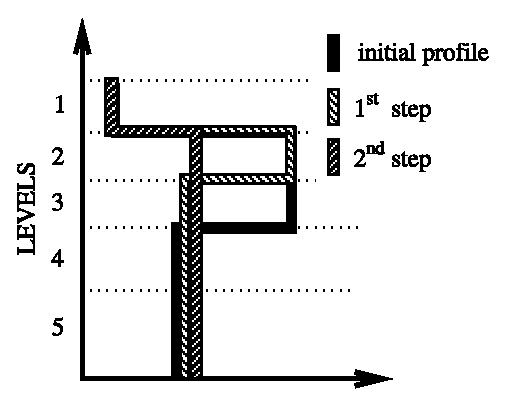
\includegraphics[width=0.90\textwidth]{Fig_npc}
\caption{  \protect\label{fig:npc} 
Example of an unstable density profile treated by the non penetrative 
convective adjustment algorithm. $1^{st}$ step: the initial profile is checked from 
the surface to the bottom. It is found to be unstable between levels 3 and 4. 
They are mixed. The resulting $\rho$ is still larger than $\rho$(5): levels 3 to 5 
are mixed. The resulting $\rho$ is still larger than $\rho$(6): levels 3 to 6 are 
mixed. The $1^{st}$ step ends since the density profile is then stable below 
the level 3. $2^{nd}$ step: the new $\rho$ profile is checked following the same 
procedure as in $1^{st}$ step: levels 2 to 5 are mixed. The new density profile 
is checked. It is found stable: end of algorithm.}
\end{center}  	\end{figure}
%>>>>>>>>>>>>>>>>>>>>>>>>>>>>

Options are defined through the  \ngn{namzdf} namelist variables.
The non-penetrative convective adjustment is used when \np{ln\_zdfnpc}\forcode{ = .true.}. 
It is applied at each \np{nn\_npc} time step and mixes downwards instantaneously 
the statically unstable portion of the water column, but only until the density 
structure becomes neutrally stable ($i.e.$ until the mixed portion of the water 
column has \textit{exactly} the density of the water just below) \citep{Madec_al_JPO91}. 
The associated algorithm is an iterative process used in the following way 
(\autoref{fig:npc}): starting from the top of the ocean, the first instability is 
found. Assume in the following that the instability is located between levels 
$k$ and $k+1$. The temperature and salinity in the two levels are 
vertically mixed, conserving the heat and salt contents of the water column. 
The new density is then computed by a linear approximation. If the new 
density profile is still unstable between levels $k+1$ and $k+2$, levels $k$, 
$k+1$ and $k+2$ are then mixed. This process is repeated until stability is 
established below the level $k$ (the mixing process can go down to the 
ocean bottom). The algorithm is repeated to check if the density profile 
between level $k-1$ and $k$ is unstable and/or if there is no deeper instability.

This algorithm is significantly different from mixing statically unstable levels 
two by two. The latter procedure cannot converge with a finite number 
of iterations for some vertical profiles while the algorithm used in \NEMO 
converges for any profile in a number of iterations which is less than the 
number of vertical levels. This property is of paramount importance as 
pointed out by \citet{Killworth1989}: it avoids the existence of permanent 
and unrealistic static instabilities at the sea surface. This non-penetrative 
convective algorithm has been proved successful in studies of the deep 
water formation in the north-western Mediterranean Sea 
\citep{Madec_al_JPO91, Madec_al_DAO91, Madec_Crepon_Bk91}.

The current implementation has been modified in order to deal with any non linear 
equation of seawater (L. Brodeau, personnal communication). 
Two main differences have been introduced compared to the original algorithm: 
$(i)$ the stability is now checked using the Brunt-V\"{a}is\"{a}l\"{a} frequency 
(not the the difference in potential density) ; 
$(ii)$ when two levels are found unstable, their thermal and haline expansion coefficients 
are vertically mixed in the same way their temperature and salinity has been mixed.
These two modifications allow the algorithm to perform properly and accurately 
with TEOS10 or EOS-80 without having to recompute the expansion coefficients at each 
mixing iteration.

% -------------------------------------------------------------------------------------------------------------
%       Enhanced Vertical Diffusion 
% -------------------------------------------------------------------------------------------------------------
\subsection{Enhanced vertical diffusion (\protect\np{ln\_zdfevd}\forcode{ = .true.})}
\label{subsec:ZDF_evd}

%--------------------------------------------namzdf--------------------------------------------------------

\nlst{namzdf}
%--------------------------------------------------------------------------------------------------------------

Options are defined through the  \ngn{namzdf} namelist variables.
The enhanced vertical diffusion parameterisation is used when \np{ln\_zdfevd}\forcode{ = .true.}. 
In this case, the vertical eddy mixing coefficients are assigned very large values 
(a typical value is $10\;m^2s^{-1})$ in regions where the stratification is unstable 
($i.e.$ when $N^2$ the Brunt-Vais\"{a}l\"{a} frequency is negative) 
\citep{Lazar_PhD97, Lazar_al_JPO99}. This is done either on tracers only 
(\np{nn\_evdm}\forcode{ = 0}) or on both momentum and tracers (\np{nn\_evdm}\forcode{ = 1}).

In practice, where $N^2\leq 10^{-12}$, $A_T^{vT}$ and $A_T^{vS}$, and 
if \np{nn\_evdm}\forcode{ = 1}, the four neighbouring $A_u^{vm} \;\mbox{and}\;A_v^{vm}$ 
values also, are set equal to the namelist parameter \np{rn\_avevd}. A typical value 
for $rn\_avevd$ is between 1 and $100~m^2.s^{-1}$. This parameterisation of 
convective processes is less time consuming than the convective adjustment 
algorithm presented above when mixing both tracers and momentum in the 
case of static instabilities. It requires the use of an implicit time stepping on 
vertical diffusion terms (i.e. \np{ln\_zdfexp}\forcode{ = .false.}). 

Note that the stability test is performed on both \textit{before} and \textit{now} 
values of $N^2$. This removes a potential source of divergence of odd and
even time step in a leapfrog environment \citep{Leclair_PhD2010} (see \autoref{sec:STP_mLF}).

% -------------------------------------------------------------------------------------------------------------
%       Turbulent Closure Scheme 
% -------------------------------------------------------------------------------------------------------------
\subsection[Turbulent closure scheme (\protect\key{zdf}\{tke,gls,osm\})]{Turbulent Closure Scheme (\protect\key{zdftke}, \protect\key{zdfgls} or \protect\key{zdfosm})}
\label{subsec:ZDF_tcs}

The turbulent closure scheme presented in \autoref{subsec:ZDF_tke} and \autoref{subsec:ZDF_gls} 
(\key{zdftke} or \key{zdftke} is defined) in theory solves the problem of statically 
unstable density profiles. In such a case, the term corresponding to the 
destruction of turbulent kinetic energy through stratification in \autoref{eq:zdftke_e} 
or \autoref{eq:zdfgls_e} becomes a source term, since $N^2$ is negative. 
It results in large values of $A_T^{vT}$ and  $A_T^{vT}$, and also the four neighbouring 
$A_u^{vm} {and}\;A_v^{vm}$ (up to $1\;m^2s^{-1})$. These large values 
restore the static stability of the water column in a way similar to that of the 
enhanced vertical diffusion parameterisation (\autoref{subsec:ZDF_evd}). However, 
in the vicinity of the sea surface (first ocean layer), the eddy coefficients 
computed by the turbulent closure scheme do not usually exceed $10^{-2}m.s^{-1}$, 
because the mixing length scale is bounded by the distance to the sea surface. 
It can thus be useful to combine the enhanced vertical 
diffusion with the turbulent closure scheme, $i.e.$ setting the \np{ln\_zdfnpc} 
namelist parameter to true and defining the turbulent closure CPP key all together.

The KPP turbulent closure scheme already includes enhanced vertical diffusion 
in the case of convection, as governed by the variables $bvsqcon$ and $difcon$ 
found in \mdl{zdfkpp}, therefore \np{ln\_zdfevd}\forcode{ = .false.} should be used with the KPP 
scheme. %gm%  + one word on non local flux with KPP scheme trakpp.F90 module...

% ================================================================
% Double Diffusion Mixing
% ================================================================
\section{Double diffusion mixing (\protect\key{zdfddm})}
\label{sec:ZDF_ddm}

%-------------------------------------------namzdf_ddm-------------------------------------------------
%
%\nlst{namzdf_ddm}
%--------------------------------------------------------------------------------------------------------------

Options are defined through the  \ngn{namzdf\_ddm} namelist variables.
Double diffusion occurs when relatively warm, salty water overlies cooler, fresher 
water, or vice versa. The former condition leads to salt fingering and the latter 
to diffusive convection. Double-diffusive phenomena contribute to diapycnal 
mixing in extensive regions of the ocean.  \citet{Merryfield1999} include a 
parameterisation of such phenomena in a global ocean model and show that 
it leads to relatively minor changes in circulation but exerts significant regional 
influences on temperature and salinity. This parameterisation has been 
introduced in \mdl{zdfddm} module and is controlled by the \key{zdfddm} CPP key.

Diapycnal mixing of S and T are described by diapycnal diffusion coefficients 
\begin{align*} % \label{eq:zdfddm_Kz}
    &A^{vT} = A_o^{vT}+A_f^{vT}+A_d^{vT}	\\
    &A^{vS} = A_o^{vS}+A_f^{vS}+A_d^{vS}
\end{align*}
where subscript $f$ represents mixing by salt fingering, $d$ by diffusive convection, 
and $o$ by processes other than double diffusion. The rates of double-diffusive 
mixing depend on the buoyancy ratio $R_\rho = \alpha \partial_z T / \beta \partial_z S$, 
where $\alpha$ and $\beta$ are coefficients of thermal expansion and saline 
contraction (see \autoref{subsec:TRA_eos}). To represent mixing of $S$ and $T$ by salt 
fingering, we adopt the diapycnal diffusivities suggested by Schmitt (1981):
\begin{align} \label{eq:zdfddm_f}
A_f^{vS} &= 	\begin{cases}
	\frac{A^{\ast v}}{1+(R_\rho / R_c)^n   } &\text{if  $R_\rho > 1$ and $N^2>0$ } \\
	0 				  					    &\text{otherwise} 
				\end{cases}   
\\ 		    \label{eq:zdfddm_f_T}
A_f^{vT} &= 0.7 \ A_f^{vS} / R_\rho 
\end{align}

%>>>>>>>>>>>>>>>>>>>>>>>>>>>>
\begin{figure}[!t]   \begin{center}
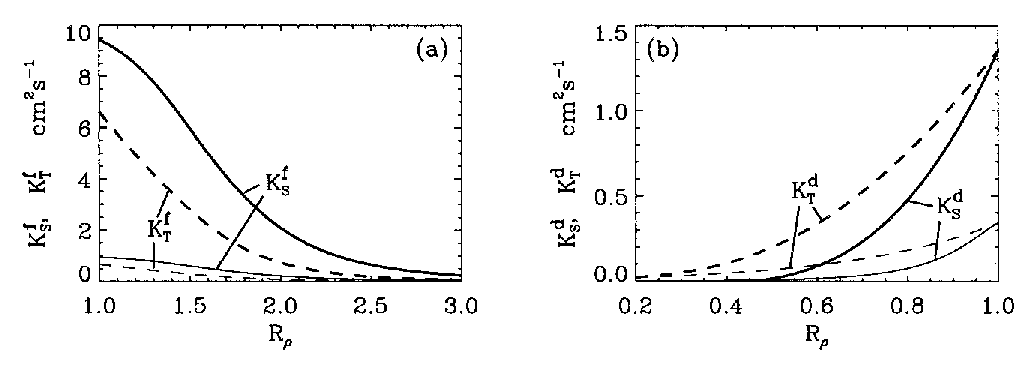
\includegraphics[width=0.99\textwidth]{Fig_zdfddm}
\caption{  \protect\label{fig:zdfddm}
From \citet{Merryfield1999} : (a) Diapycnal diffusivities $A_f^{vT}$ 
and $A_f^{vS}$ for temperature and salt in regions of salt fingering. Heavy 
curves denote $A^{\ast v} = 10^{-3}~m^2.s^{-1}$ and thin curves 
$A^{\ast v} = 10^{-4}~m^2.s^{-1}$ ; (b) diapycnal diffusivities $A_d^{vT}$ and 
$A_d^{vS}$ for temperature and salt in regions of diffusive convection. Heavy 
curves denote the Federov parameterisation and thin curves the Kelley 
parameterisation. The latter is not implemented in \NEMO. }
\end{center}    \end{figure}
%>>>>>>>>>>>>>>>>>>>>>>>>>>>>

The factor 0.7 in \autoref{eq:zdfddm_f_T} reflects the measured ratio 
$\alpha F_T /\beta F_S \approx  0.7$ of buoyancy flux of heat to buoyancy 
flux of salt ($e.g.$, \citet{McDougall_Taylor_JMR84}). Following  \citet{Merryfield1999}, 
we adopt $R_c = 1.6$, $n = 6$, and $A^{\ast v} = 10^{-4}~m^2.s^{-1}$.

To represent mixing of S and T by diffusive layering,  the diapycnal diffusivities suggested by Federov (1988) is used: 
\begin{align} 	\label{eq:zdfddm_d}
A_d^{vT} &= 	\begin{cases}
	1.3635 \, \exp{\left( 4.6\, \exp{ \left[  -0.54\,( R_{\rho}^{-1} - 1 )  \right] }    \right)}
									&\text{if  $0<R_\rho < 1$ and $N^2>0$ } \\
	0 								&\text{otherwise} 
				\end{cases}   
\\   			\label{eq:zdfddm_d_S}
A_d^{vS} &= 	\begin{cases}
	A_d^{vT}\ \left( 1.85\,R_{\rho} - 0.85 \right)
									&\text{if  $0.5 \leq R_\rho<1$ and $N^2>0$ } \\
	A_d^{vT} \ 0.15 \ R_\rho
									&\text{if  $\ \ 0 < R_\rho<0.5$ and $N^2>0$ } \\
	0 								&\text{otherwise} 
				\end{cases}   
\end{align}

The dependencies of \autoref{eq:zdfddm_f} to \autoref{eq:zdfddm_d_S} on $R_\rho$ 
are illustrated in \autoref{fig:zdfddm}. Implementing this requires computing 
$R_\rho$ at each grid point on every time step. This is done in \mdl{eosbn2} at the 
same time as $N^2$ is computed. This avoids duplication in the computation of 
$\alpha$ and $\beta$ (which is usually quite expensive).

% ================================================================
% Bottom Friction
% ================================================================
\section{Bottom and top friction (\protect\mdl{zdfbfr})}
\label{sec:ZDF_bfr}

%--------------------------------------------nambfr--------------------------------------------------------
%
%\nlst{nambfr}
%--------------------------------------------------------------------------------------------------------------

Options to define the top and bottom friction are defined through the  \ngn{nambfr} namelist variables.
The bottom friction represents the friction generated by the bathymetry. 
The top friction represents the friction generated by the ice shelf/ocean interface. 
As the friction processes at the top and bottom are treated in similar way, 
only the bottom friction is described in detail below.


Both the surface momentum flux (wind stress) and the bottom momentum 
flux (bottom friction) enter the equations as a condition on the vertical 
diffusive flux. For the bottom boundary layer, one has:
\begin{equation} \label{eq:zdfbfr_flux}
A^{vm} \left( \partial {\textbf U}_h / \partial z \right) = {{\cal F}}_h^{\textbf U}
\end{equation}
where ${\cal F}_h^{\textbf U}$ is represents the downward flux of horizontal momentum 
outside the logarithmic turbulent boundary layer (thickness of the order of 
1~m in the ocean). How ${\cal F}_h^{\textbf U}$ influences the interior depends on the 
vertical resolution of the model near the bottom relative to the Ekman layer 
depth. For example, in order to obtain an Ekman layer depth 
$d = \sqrt{2\;A^{vm}} / f = 50$~m, one needs a vertical diffusion coefficient 
$A^{vm} = 0.125$~m$^2$s$^{-1}$ (for a Coriolis frequency 
$f = 10^{-4}$~m$^2$s$^{-1}$). With a background diffusion coefficient 
$A^{vm} = 10^{-4}$~m$^2$s$^{-1}$, the Ekman layer depth is only 1.4~m. 
When the vertical mixing coefficient is this small, using a flux condition is 
equivalent to entering the viscous forces (either wind stress or bottom friction) 
as a body force over the depth of the top or bottom model layer. To illustrate 
this, consider the equation for $u$ at $k$, the last ocean level:
\begin{equation} \label{eq:zdfbfr_flux2}
\frac{\partial u_k}{\partial t} = \frac{1}{e_{3u}} \left[ \frac{A_{uw}^{vm}}{e_{3uw}} \delta_{k+1/2}\;[u] - {\cal F}^u_h \right] \approx - \frac{{\cal F}^u_{h}}{e_{3u}}
\end{equation}
If the bottom layer thickness is 200~m, the Ekman transport will 
be distributed over that depth. On the other hand, if the vertical resolution 
is high (1~m or less) and a turbulent closure model is used, the turbulent 
Ekman layer will be represented explicitly by the model. However, the 
logarithmic layer is never represented in current primitive equation model 
applications: it is \emph{necessary} to parameterize the flux ${\cal F}^u_h $. 
Two choices are available in \NEMO: a linear and a quadratic bottom friction. 
Note that in both cases, the rotation between the interior velocity and the 
bottom friction is neglected in the present release of \NEMO.

In the code, the bottom friction is imposed by adding the trend due to the bottom 
friction to the general momentum trend in \mdl{dynbfr}. For the time-split surface 
pressure gradient algorithm, the momentum trend due to the barotropic component 
needs to be handled separately. For this purpose it is convenient to compute and 
store coefficients which can be simply combined with bottom velocities and geometric 
values to provide the momentum trend due to bottom friction. 
These coefficients are computed in \mdl{zdfbfr} and generally take the form 
$c_b^{\textbf U}$ where:
\begin{equation} \label{eq:zdfbfr_bdef}
\frac{\partial {\textbf U_h}}{\partial t} = 
  - \frac{{\cal F}^{\textbf U}_{h}}{e_{3u}} = \frac{c_b^{\textbf U}}{e_{3u}} \;{\textbf U}_h^b
\end{equation}
where $\textbf{U}_h^b = (u_b\;,\;v_b)$ is the near-bottom, horizontal, ocean velocity.

% -------------------------------------------------------------------------------------------------------------
%       Linear Bottom Friction
% -------------------------------------------------------------------------------------------------------------
\subsection{Linear bottom friction (\protect\np{nn\_botfr}\forcode{ = 0..1})}
\label{subsec:ZDF_bfr_linear}

The linear bottom friction parameterisation (including the special case 
of a free-slip condition) assumes that the bottom friction 
is proportional to the interior velocity (i.e. the velocity of the last 
model level):
\begin{equation} \label{eq:zdfbfr_linear}
{\cal F}_h^\textbf{U} = \frac{A^{vm}}{e_3} \; \frac{\partial \textbf{U}_h}{\partial k} = r \; \textbf{U}_h^b
\end{equation}
where $r$ is a friction coefficient expressed in ms$^{-1}$. 
This coefficient is generally estimated by setting a typical decay time 
$\tau$ in the deep ocean, 
and setting $r = H / \tau$, where $H$ is the ocean depth. Commonly accepted 
values of $\tau$ are of the order of 100 to 200 days \citep{Weatherly_JMR84}. 
A value $\tau^{-1} = 10^{-7}$~s$^{-1}$ equivalent to 115 days, is usually used 
in quasi-geostrophic models. One may consider the linear friction as an 
approximation of quadratic friction, $r \approx 2\;C_D\;U_{av}$ (\citet{Gill1982}, 
Eq. 9.6.6). For example, with a drag coefficient $C_D = 0.002$, a typical speed 
of tidal currents of $U_{av} =0.1$~m\;s$^{-1}$, and assuming an ocean depth 
$H = 4000$~m, the resulting friction coefficient is $r = 4\;10^{-4}$~m\;s$^{-1}$. 
This is the default value used in \NEMO. It corresponds to a decay time scale 
of 115~days. It can be changed by specifying \np{rn\_bfri1} (namelist parameter).

For the linear friction case the coefficients defined in the general 
expression \autoref{eq:zdfbfr_bdef} are: 
\begin{equation} \label{eq:zdfbfr_linbfr_b}
\begin{split}
 c_b^u &= - r\\
 c_b^v &= - r\\
\end{split}
\end{equation}
When \np{nn\_botfr}\forcode{ = 1}, the value of $r$ used is \np{rn\_bfri1}. 
Setting \np{nn\_botfr}\forcode{ = 0} is equivalent to setting $r=0$ and leads to a free-slip 
bottom boundary condition. These values are assigned in \mdl{zdfbfr}. 
From v3.2 onwards there is support for local enhancement of these values 
via an externally defined 2D mask array (\np{ln\_bfr2d}\forcode{ = .true.}) given
in the \ifile{bfr\_coef} input NetCDF file. The mask values should vary from 0 to 1. 
Locations with a non-zero mask value will have the friction coefficient increased 
by $mask\_value$*\np{rn\_bfrien}*\np{rn\_bfri1}.

% -------------------------------------------------------------------------------------------------------------
%       Non-Linear Bottom Friction
% -------------------------------------------------------------------------------------------------------------
\subsection{Non-linear bottom friction (\protect\np{nn\_botfr}\forcode{ = 2})}
\label{subsec:ZDF_bfr_nonlinear}

The non-linear bottom friction parameterisation assumes that the bottom 
friction is quadratic: 
\begin{equation} \label{eq:zdfbfr_nonlinear}
{\cal F}_h^\textbf{U} = \frac{A^{vm}}{e_3 }\frac{\partial \textbf {U}_h 
}{\partial k}=C_D \;\sqrt {u_b ^2+v_b ^2+e_b } \;\; \textbf {U}_h^b 
\end{equation}
where $C_D$ is a drag coefficient, and $e_b $ a bottom turbulent kinetic energy 
due to tides, internal waves breaking and other short time scale currents. 
A typical value of the drag coefficient is $C_D = 10^{-3} $. As an example, 
the CME experiment \citep{Treguier_JGR92} uses $C_D = 10^{-3}$ and 
$e_b = 2.5\;10^{-3}$m$^2$\;s$^{-2}$, while the FRAM experiment \citep{Killworth1992} 
uses $C_D = 1.4\;10^{-3}$ and $e_b =2.5\;\;10^{-3}$m$^2$\;s$^{-2}$. 
The CME choices have been set as default values (\np{rn\_bfri2} and \np{rn\_bfeb2} 
namelist parameters).

As for the linear case, the bottom friction is imposed in the code by 
adding the trend due to the bottom friction to the general momentum trend 
in \mdl{dynbfr}.
For the non-linear friction case the terms
computed in \mdl{zdfbfr}  are: 
\begin{equation} \label{eq:zdfbfr_nonlinbfr}
\begin{split}
 c_b^u &= - \; C_D\;\left[ u^2 + \left(\bar{\bar{v}}^{i+1,j}\right)^2 + e_b \right]^{1/2}\\
 c_b^v &= - \; C_D\;\left[  \left(\bar{\bar{u}}^{i,j+1}\right)^2 + v^2 + e_b \right]^{1/2}\\
\end{split}
\end{equation}

The coefficients that control the strength of the non-linear bottom friction are
initialised as namelist parameters: $C_D$= \np{rn\_bfri2}, and $e_b$ =\np{rn\_bfeb2}.
Note for applications which treat tides explicitly a low or even zero value of
\np{rn\_bfeb2} is recommended. From v3.2 onwards a local enhancement of $C_D$ is possible
via an externally defined 2D mask array (\np{ln\_bfr2d}\forcode{ = .true.}).  This works in the same way
as for the linear bottom friction case with non-zero masked locations increased by
$mask\_value$*\np{rn\_bfrien}*\np{rn\_bfri2}.

% -------------------------------------------------------------------------------------------------------------
%       Bottom Friction Log-layer
% -------------------------------------------------------------------------------------------------------------
\subsection[Log-layer btm frict enhncmnt (\protect\np{nn\_botfr}\forcode{ = 2}, \protect\np{ln\_loglayer}\forcode{ = .true.})]
				{Log-layer bottom friction enhancement (\protect\np{nn\_botfr}\forcode{ = 2}, \protect\np{ln\_loglayer}\forcode{ = .true.})}
\label{subsec:ZDF_bfr_loglayer}

In the non-linear bottom friction case, the drag coefficient, $C_D$, can be optionally
enhanced using a "law of the wall" scaling. If  \np{ln\_loglayer} = .true., $C_D$ is no
longer constant but is related to the thickness of the last wet layer in each column by:

\begin{equation}
C_D = \left ( {\kappa \over {\rm log}\left ( 0.5e_{3t}/rn\_bfrz0 \right ) } \right )^2
\end{equation}

\noindent where $\kappa$ is the von-Karman constant and \np{rn\_bfrz0} is a roughness
length provided via the namelist.

For stability, the drag coefficient is bounded such that it is kept greater or equal to
the base \np{rn\_bfri2} value and it is not allowed to exceed the value of an additional
namelist parameter: \np{rn\_bfri2\_max}, i.e.:

\begin{equation}
rn\_bfri2 \leq C_D \leq rn\_bfri2\_max
\end{equation}

\noindent Note also that a log-layer enhancement can also be applied to the top boundary
friction if under ice-shelf cavities are in use (\np{ln\_isfcav}\forcode{ = .true.}).  In this case, the
relevant namelist parameters are \np{rn\_tfrz0}, \np{rn\_tfri2}
and \np{rn\_tfri2\_max}.

% -------------------------------------------------------------------------------------------------------------
%       Bottom Friction stability
% -------------------------------------------------------------------------------------------------------------
\subsection{Bottom friction stability considerations}
\label{subsec:ZDF_bfr_stability}

Some care needs to exercised over the choice of parameters to ensure that the
implementation of bottom friction does not induce numerical instability. For 
the purposes of stability analysis, an approximation to \autoref{eq:zdfbfr_flux2}
is:
\begin{equation} \label{eq:Eqn_bfrstab}
\begin{split}
 \Delta u &= -\frac{{{\cal F}_h}^u}{e_{3u}}\;2 \rdt    \\
               &= -\frac{ru}{e_{3u}}\;2\rdt\\
\end{split}
\end{equation}
\noindent where linear bottom friction and a leapfrog timestep have been assumed. 
To ensure that the bottom friction cannot reverse the direction of flow it is necessary to have:
\begin{equation}
 |\Delta u| < \;|u| 
\end{equation}
\noindent which, using \autoref{eq:Eqn_bfrstab}, gives:
\begin{equation}
r\frac{2\rdt}{e_{3u}} < 1 \qquad  \Rightarrow \qquad r < \frac{e_{3u}}{2\rdt}\\
\end{equation}
This same inequality can also be derived in the non-linear bottom friction case 
if a velocity of 1 m.s$^{-1}$ is assumed. Alternatively, this criterion can be 
rearranged to suggest a minimum bottom box thickness to ensure stability:
\begin{equation}
e_{3u} > 2\;r\;\rdt
\end{equation}
\noindent which it may be necessary to impose if partial steps are being used. 
For example, if $|u| = 1$ m.s$^{-1}$, $rdt = 1800$ s, $r = 10^{-3}$ then
$e_{3u}$ should be greater than 3.6 m. For most applications, with physically
sensible parameters these restrictions should not be of concern. But 
caution may be necessary if attempts are made to locally enhance the bottom
friction parameters. 
To ensure stability limits are imposed on the bottom friction coefficients both during 
initialisation and at each time step. Checks at initialisation are made in \mdl{zdfbfr} 
(assuming a 1 m.s$^{-1}$ velocity in the non-linear case).
The number of breaches of the stability criterion are reported as well as the minimum 
and maximum values that have been set. The criterion is also checked at each time step, 
using the actual velocity, in \mdl{dynbfr}. Values of the bottom friction coefficient are 
reduced as necessary to ensure stability; these changes are not reported.

Limits on the bottom friction coefficient are not imposed if the user has elected to
handle the bottom friction implicitly (see \autoref{subsec:ZDF_bfr_imp}). The number of potential
breaches of the explicit stability criterion are still reported for information purposes.

% -------------------------------------------------------------------------------------------------------------
%       Implicit Bottom Friction
% -------------------------------------------------------------------------------------------------------------
\subsection{Implicit bottom friction (\protect\np{ln\_bfrimp}\forcode{ = .true.})}
\label{subsec:ZDF_bfr_imp}

An optional implicit form of bottom friction has been implemented to improve
model stability. We recommend this option for shelf sea and coastal ocean applications, especially 
for split-explicit time splitting. This option can be invoked by setting \np{ln\_bfrimp} 
to \forcode{.true.} in the \textit{nambfr} namelist. This option requires \np{ln\_zdfexp} to be \forcode{.false.} 
in the \textit{namzdf} namelist. 

This implementation is realised in \mdl{dynzdf\_imp} and \mdl{dynspg\_ts}. In \mdl{dynzdf\_imp}, the 
bottom boundary condition is implemented implicitly.

\begin{equation} \label{eq:dynzdf_bfr}
\left.{\left( {\frac{A^{vm} }{e_3 }\ \frac{\partial \textbf{U}_h}{\partial k}} \right)} \right|_{mbk}
	 = \binom{c_{b}^{u}u^{n+1}_{mbk}}{c_{b}^{v}v^{n+1}_{mbk}}
\end{equation}

where $mbk$ is the layer number of the bottom wet layer. superscript $n+1$ means the velocity used in the
friction formula is to be calculated, so, it is implicit.

If split-explicit time splitting is used, care must be taken to avoid the double counting of
the bottom friction in the 2-D barotropic momentum equations. As NEMO only updates the barotropic 
pressure gradient and Coriolis' forcing terms in the 2-D barotropic calculation, we need to remove
the bottom friction induced by these two terms which has been included in the 3-D momentum trend 
and update it with the latest value. On the other hand, the bottom friction contributed by the
other terms (e.g. the advection term, viscosity term) has been included in the 3-D momentum equations
and should not be added in the 2-D barotropic mode.

The implementation of the implicit bottom friction in \mdl{dynspg\_ts} is done in two steps as the
following:

\begin{equation} \label{eq:dynspg_ts_bfr1}
\frac{\textbf{U}_{med}-\textbf{U}^{m-1}}{2\Delta t}=-g\nabla\eta-f\textbf{k}\times\textbf{U}^{m}+c_{b}
\left(\textbf{U}_{med}-\textbf{U}^{m-1}\right)
\end{equation}
\begin{equation} \label{eq:dynspg_ts_bfr2}
\frac{\textbf{U}^{m+1}-\textbf{U}_{med}}{2\Delta t}=\textbf{T}+
\left(g\nabla\eta^{'}+f\textbf{k}\times\textbf{U}^{'}\right)-
2\Delta t_{bc}c_{b}\left(g\nabla\eta^{'}+f\textbf{k}\times\textbf{u}_{b}\right)
\end{equation}

where $\textbf{T}$ is the vertical integrated 3-D momentum trend. We assume the leap-frog time-stepping
is used here. $\Delta t$ is the barotropic mode time step and $\Delta t_{bc}$ is the baroclinic mode time step.
 $c_{b}$ is the friction coefficient. $\eta$ is the sea surface level calculated in the barotropic loops
while $\eta^{'}$ is the sea surface level used in the 3-D baroclinic mode. $\textbf{u}_{b}$ is the bottom
layer horizontal velocity.




% -------------------------------------------------------------------------------------------------------------
%       Bottom Friction with split-explicit time splitting
% -------------------------------------------------------------------------------------------------------------
\subsection[Bottom friction w/ split-explicit time splitting (\protect\np{ln\_bfrimp})]
				{Bottom friction with split-explicit time splitting (\protect\np{ln\_bfrimp})}
\label{subsec:ZDF_bfr_ts}

When calculating the momentum trend due to bottom friction in \mdl{dynbfr}, the
bottom velocity at the before time step is used. This velocity includes both the
baroclinic and barotropic components which is appropriate when using either the
explicit or filtered surface pressure gradient algorithms (\key{dynspg\_exp} or 
\key{dynspg\_flt}). Extra attention is required, however, when using 
split-explicit time stepping (\key{dynspg\_ts}). In this case the free surface 
equation is solved with a small time step \np{rn\_rdt}/\np{nn\_baro}, while the three 
dimensional prognostic variables are solved with the longer time step 
of \np{rn\_rdt} seconds. The trend in the barotropic momentum due to bottom 
friction appropriate to this method is that given by the selected parameterisation 
($i.e.$ linear or non-linear bottom friction) computed with the evolving velocities 
at each barotropic timestep. 

In the case of non-linear bottom friction, we have elected to partially linearise 
the problem by keeping the coefficients fixed throughout the barotropic 
time-stepping to those computed in \mdl{zdfbfr} using the now timestep. 
This decision allows an efficient use of the $c_b^{\vect{U}}$ coefficients to:

\begin{enumerate}
\item On entry to \rou{dyn\_spg\_ts}, remove the contribution of the before
barotropic velocity to the bottom friction component of the vertically
integrated momentum trend. Note the same stability check that is carried out 
on the bottom friction coefficient in \mdl{dynbfr} has to be applied here to
ensure that the trend removed matches that which was added in \mdl{dynbfr}.
\item At each barotropic step, compute the contribution of the current barotropic
velocity to the trend due to bottom friction. Add this contribution to the
vertically integrated momentum trend. This contribution is handled implicitly which
eliminates the need to impose a stability criteria on the values of the bottom friction
coefficient within the barotropic loop. 
\end{enumerate}

Note that the use of an implicit formulation within the barotropic loop
for the bottom friction trend means that any limiting of the bottom friction coefficient 
in \mdl{dynbfr} does not adversely affect the solution when using split-explicit time 
splitting. This is because the major contribution to bottom friction is likely to come from 
the barotropic component which uses the unrestricted value of the coefficient. However, if the
limiting is thought to be having a major effect (a more likely prospect in coastal and shelf seas
applications) then the fully implicit form of the bottom friction should be used (see \autoref{subsec:ZDF_bfr_imp} ) 
which can be selected by setting \np{ln\_bfrimp} $=$ \forcode{.true.}.

Otherwise, the implicit formulation takes the form:
\begin{equation} \label{eq:zdfbfr_implicitts}
 \bar{U}^{t+ \rdt} = \; \left [ \bar{U}^{t-\rdt}\; + 2 \rdt\;RHS \right ] / \left [ 1 - 2 \rdt \;c_b^{u} / H_e \right ]  
\end{equation}
where $\bar U$ is the barotropic velocity, $H_e$ is the full depth (including sea surface height), 
$c_b^u$ is the bottom friction coefficient as calculated in \rou{zdf\_bfr} and $RHS$ represents 
all the components to the vertically integrated momentum trend except for that due to bottom friction.




% ================================================================
% Tidal Mixing
% ================================================================
\section{Tidal mixing (\protect\key{zdftmx})}
\label{sec:ZDF_tmx}

%--------------------------------------------namzdf_tmx--------------------------------------------------
%
%\nlst{namzdf_tmx}
%--------------------------------------------------------------------------------------------------------------


% -------------------------------------------------------------------------------------------------------------
%        Bottom intensified tidal mixing 
% -------------------------------------------------------------------------------------------------------------
\subsection{Bottom intensified tidal mixing}
\label{subsec:ZDF_tmx_bottom}

Options are defined through the  \ngn{namzdf\_tmx} namelist variables.
The parameterization of tidal mixing follows the general formulation for 
the vertical eddy diffusivity proposed by \citet{St_Laurent_al_GRL02} and 
first introduced in an OGCM by \citep{Simmons_al_OM04}. 
In this formulation an additional vertical diffusivity resulting from internal tide breaking, 
$A^{vT}_{tides}$ is expressed as a function of $E(x,y)$, the energy transfer from barotropic 
tides to baroclinic tides : 
\begin{equation} \label{eq:Ktides}
A^{vT}_{tides} =  q \,\Gamma \,\frac{ E(x,y) \, F(z) }{ \rho \, N^2 }
\end{equation}
where $\Gamma$ is the mixing efficiency, $N$ the Brunt-Vais\"{a}l\"{a} frequency 
(see \autoref{subsec:TRA_bn2}), $\rho$ the density, $q$ the tidal dissipation efficiency, 
and $F(z)$ the vertical structure function. 

The mixing efficiency of turbulence is set by $\Gamma$ (\np{rn\_me} namelist parameter)
and is usually taken to be the canonical value of $\Gamma = 0.2$ (Osborn 1980). 
The tidal dissipation efficiency is given by the parameter $q$ (\np{rn\_tfe} namelist parameter) 
represents the part of the internal wave energy flux $E(x, y)$ that is dissipated locally, 
with the remaining $1-q$ radiating away as low mode internal waves and 
contributing to the background internal wave field. A value of $q=1/3$ is typically used  
\citet{St_Laurent_al_GRL02}.
The vertical structure function $F(z)$ models the distribution of the turbulent mixing in the vertical. 
It is implemented as a simple exponential decaying upward away from the bottom, 
with a vertical scale of $h_o$ (\np{rn\_htmx} namelist parameter, with a typical value of $500\,m$) \citep{St_Laurent_Nash_DSR04}, 
\begin{equation} \label{eq:Fz}
F(i,j,k) = \frac{ e^{ -\frac{H+z}{h_o} } }{ h_o \left( 1- e^{ -\frac{H}{h_o} } \right) }
\end{equation}
and is normalized so that vertical integral over the water column is unity. 

The associated vertical viscosity is calculated from the vertical 
diffusivity assuming a Prandtl number of 1, $i.e.$ $A^{vm}_{tides}=A^{vT}_{tides}$. 
In the limit of $N \rightarrow 0$ (or becoming negative), the vertical diffusivity 
is capped at $300\,cm^2/s$ and impose a lower limit on $N^2$ of \np{rn\_n2min} 
usually set to $10^{-8} s^{-2}$. These bounds are usually rarely encountered.

The internal wave energy map, $E(x, y)$ in \autoref{eq:Ktides}, is derived 
from a barotropic model of the tides utilizing a parameterization of the 
conversion of barotropic tidal energy into internal waves. 
The essential goal of the parameterization is to represent the momentum 
exchange between the barotropic tides and the unrepresented internal waves 
induced by the tidal flow over rough topography in a stratified ocean. 
In the current version of \NEMO, the map is built from the output of 
the barotropic global ocean tide model MOG2D-G \citep{Carrere_Lyard_GRL03}.
This model provides the dissipation associated with internal wave energy for the M2 and K1 
tides component (\autoref{fig:ZDF_M2_K1_tmx}). The S2 dissipation is simply approximated
as being $1/4$ of the M2 one. The internal wave energy is thus : $E(x, y) = 1.25 E_{M2} + E_{K1}$. 
Its global mean value is $1.1$ TW, in agreement with independent estimates 
\citep{Egbert_Ray_Nat00, Egbert_Ray_JGR01}. 

%>>>>>>>>>>>>>>>>>>>>>>>>>>>>
\begin{figure}[!t] 	\begin{center}
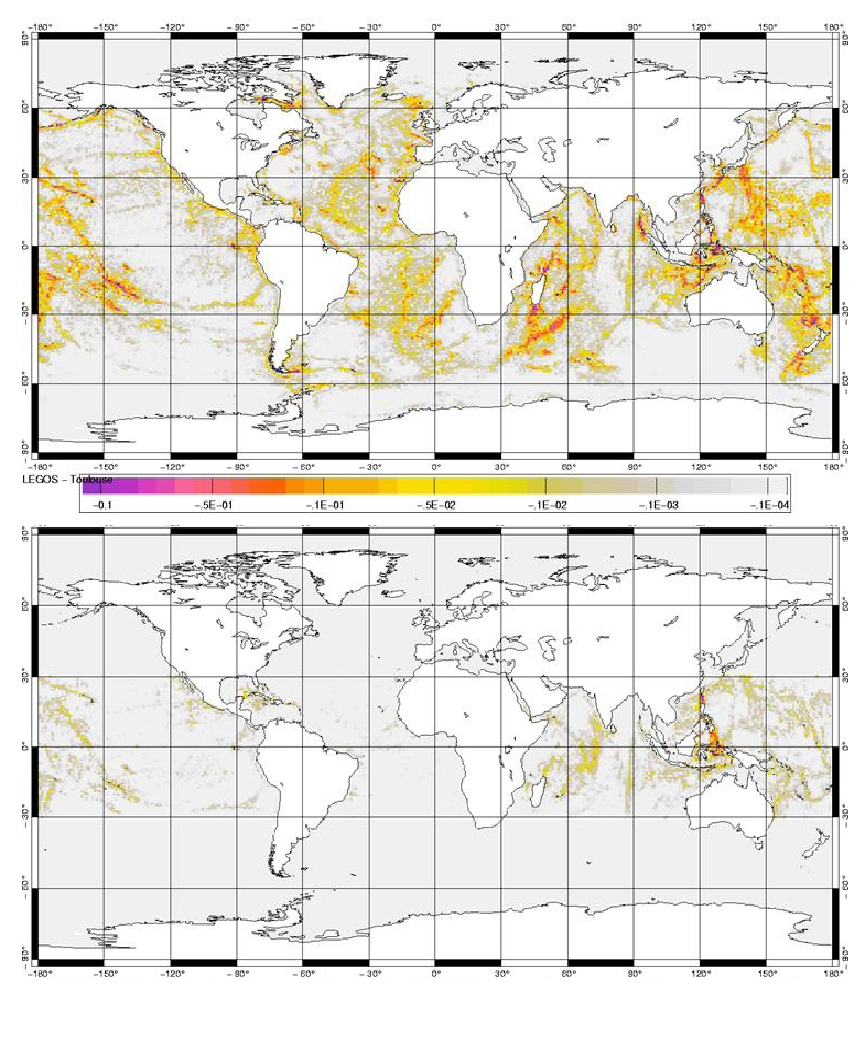
\includegraphics[width=0.90\textwidth]{Fig_ZDF_M2_K1_tmx}
\caption{  \protect\label{fig:ZDF_M2_K1_tmx} 
(a) M2 and (b) K1 internal wave drag energy from \citet{Carrere_Lyard_GRL03} ($W/m^2$). }
\end{center}  	\end{figure}
%>>>>>>>>>>>>>>>>>>>>>>>>>>>> 
 
% -------------------------------------------------------------------------------------------------------------
%        Indonesian area specific treatment 
% -------------------------------------------------------------------------------------------------------------
\subsection{Indonesian area specific treatment (\protect\np{ln\_zdftmx\_itf})}
\label{subsec:ZDF_tmx_itf}

When the Indonesian Through Flow (ITF) area is included in the model domain,
a specific treatment of tidal induced mixing in this area can be used. 
It is activated through the namelist logical \np{ln\_tmx\_itf}, and the user must provide
an input NetCDF file, \ifile{mask\_itf}, which contains a mask array defining the ITF area
where the specific treatment is applied.

When \np{ln\_tmx\_itf}\forcode{ = .true.}, the two key parameters $q$ and $F(z)$ are adjusted following 
the parameterisation developed by \citet{Koch-Larrouy_al_GRL07}:

First, the Indonesian archipelago is a complex geographic region 
with a series of large, deep, semi-enclosed basins connected via 
numerous narrow straits. Once generated, internal tides remain 
confined within this semi-enclosed area and hardly radiate away. 
Therefore all the internal tides energy is consumed within this area. 
So it is assumed that $q = 1$, $i.e.$ all the energy generated is available for mixing.
Note that for test purposed, the ITF tidal dissipation efficiency is a 
namelist parameter (\np{rn\_tfe\_itf}). A value of $1$ or close to is
this recommended for this parameter.

Second, the vertical structure function, $F(z)$, is no more associated
with a bottom intensification of the mixing, but with a maximum of 
energy available within the thermocline. \citet{Koch-Larrouy_al_GRL07} 
have suggested that the vertical distribution of the energy dissipation 
proportional to $N^2$ below the core of the thermocline and to $N$ above. 
The resulting $F(z)$ is:
\begin{equation} \label{eq:Fz_itf}
F(i,j,k) \sim     \left\{ \begin{aligned}
\frac{q\,\Gamma E(i,j) } {\rho N \, \int N     dz}    \qquad \text{when $\partial_z N < 0$} \\
\frac{q\,\Gamma E(i,j) } {\rho     \, \int N^2 dz}    \qquad \text{when $\partial_z N > 0$}
                      \end{aligned} \right.
\end{equation}

Averaged over the ITF area, the resulting tidal mixing coefficient is $1.5\,cm^2/s$, 
which agrees with the independent estimates inferred from observations. 
Introduced in a regional OGCM, the parameterization improves the water mass 
characteristics in the different Indonesian seas, suggesting that the horizontal 
and vertical distributions of the mixing are adequately prescribed 
\citep{Koch-Larrouy_al_GRL07, Koch-Larrouy_al_OD08a, Koch-Larrouy_al_OD08b}.
Note also that such a parameterisation has a significant impact on the behaviour 
of global coupled GCMs \citep{Koch-Larrouy_al_CD10}.


% ================================================================
% Internal wave-driven mixing
% ================================================================
\section{Internal wave-driven mixing (\protect\key{zdftmx\_new})}
\label{sec:ZDF_tmx_new}

%--------------------------------------------namzdf_tmx_new------------------------------------------
%
%\nlst{namzdf_tmx_new}
%--------------------------------------------------------------------------------------------------------------

The parameterization of mixing induced by breaking internal waves is a generalization 
of the approach originally proposed by \citet{St_Laurent_al_GRL02}. 
A three-dimensional field of internal wave energy dissipation $\epsilon(x,y,z)$ is first constructed, 
and the resulting diffusivity is obtained as 
\begin{equation} \label{eq:Kwave}
A^{vT}_{wave} =  R_f \,\frac{ \epsilon }{ \rho \, N^2 }
\end{equation}
where $R_f$ is the mixing efficiency and $\epsilon$ is a specified three dimensional distribution 
of the energy available for mixing. If the \np{ln\_mevar} namelist parameter is set to false, 
the mixing efficiency is taken as constant and equal to 1/6 \citep{Osborn_JPO80}. 
In the opposite (recommended) case, $R_f$ is instead a function of the turbulence intensity parameter 
$Re_b = \frac{ \epsilon}{\nu \, N^2}$, with $\nu$ the molecular viscosity of seawater, 
following the model of \cite{Bouffard_Boegman_DAO2013} 
and the implementation of \cite{de_lavergne_JPO2016_efficiency}.
Note that $A^{vT}_{wave}$ is bounded by $10^{-2}\,m^2/s$, a limit that is often reached when the mixing efficiency is constant.

In addition to the mixing efficiency, the ratio of salt to heat diffusivities can chosen to vary 
as a function of $Re_b$ by setting the \np{ln\_tsdiff} parameter to true, a recommended choice). 
This parameterization of differential mixing, due to \cite{Jackson_Rehmann_JPO2014}, 
is implemented as in \cite{de_lavergne_JPO2016_efficiency}.

The three-dimensional distribution of the energy available for mixing, $\epsilon(i,j,k)$, is constructed 
from three static maps of column-integrated internal wave energy dissipation, $E_{cri}(i,j)$, 
$E_{pyc}(i,j)$, and $E_{bot}(i,j)$, combined to three corresponding vertical structures 
(de Lavergne et al., in prep):
\begin{align*}
F_{cri}(i,j,k) &\propto e^{-h_{ab} / h_{cri} }\\
F_{pyc}(i,j,k) &\propto N^{n\_p}\\
F_{bot}(i,j,k) &\propto N^2 \, e^{- h_{wkb} / h_{bot} }
\end{align*} 
In the above formula, $h_{ab}$ denotes the height above bottom, 
$h_{wkb}$ denotes the WKB-stretched height above bottom, defined by
\begin{equation*}
h_{wkb} = H \, \frac{ \int_{-H}^{z} N \, dz' } { \int_{-H}^{\eta} N \, dz'  } \; ,
\end{equation*}
The $n_p$ parameter (given by \np{nn\_zpyc} in \ngn{namzdf\_tmx\_new} namelist)  controls the stratification-dependence of the pycnocline-intensified dissipation. 
It can take values of 1 (recommended) or 2.
Finally, the vertical structures $F_{cri}$ and $F_{bot}$ require the specification of 
the decay scales $h_{cri}(i,j)$ and $h_{bot}(i,j)$, which are defined by two additional input maps. 
$h_{cri}$ is related to the large-scale topography of the ocean (etopo2) 
and $h_{bot}$ is a function of the energy flux $E_{bot}$, the characteristic horizontal scale of 
the abyssal hill topography \citep{Goff_JGR2010} and the latitude.

% ================================================================



\end{document}
